%%%%%%%%%% CAPITOLO DI TESI %%%%%%%%%%
%
% Capitolo "1" Capitolo 1
%
%%%%%%%%%%%%%%%%%%%%%%%%%%%%%%%%%%%%%%
\mcchap{Capitolo 1}{cap:cap1}
Qualcosa sul capitolo 1
\section{section}
Qualcosa ancora sul capitolo 1
\section{section again}
Qualcosa ancora sul capitolo 1
\subsection{subsection}
Qualcosa ancora sul capitolo 1

\section{Citazioni}
Per citare bisogna editare il file biblio/biblio.bib e aggiungere in formato bibtex la citazione poi citarla così: citazione~\cite{STORY}. 
Automaticamente verrà aggiunta alla bibliografia quando citata.

\section{Immagini}
Si possono caricare immagini ed usare reference per citarle: Fig.~\ref{fig:TDD}
\begin{figure}[H]
    \begin{flushright}
        \centering
        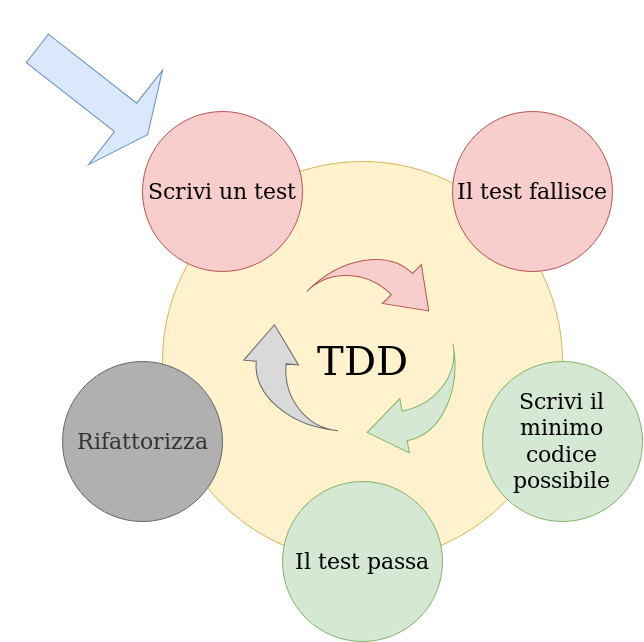
\includegraphics[width=0.4\textwidth]{imgs/TDDCycle.png}
        \caption{Ciclo del TDD}
        \label{fig:TDD}
    \end{flushright}
\end{figure}

\section{Tabelle}
Le tabelle si citano come le immagini: Tab.~\ref{tab:mlp}

\begin {table}[H]
\caption {Confronto MLP e SVM in media} \label{tab:mlp} 
\begin{center}
\begin{tabular}{|c|c|c|}
  
  \hline
  \rowcolor[gray]{.6}
  \textbf{SVM jaccard} & \textbf{MLP jaccard} & \textbf{MLP jaccard – SVM jaccard} \\
  
  \hline
  \rowcolor[gray]{.8}
  0,4275 & 0,29172 & \textcolor{red}{-0,13578}\\
  \hline
\end{tabular} 
\end{center}
\end{table}

\section{code}

Il codice può essere scritto inline List.~\ref{code:bash}:
\begin{lstlisting}[language=DebianBash, style=basic, label=code:bash, caption=sample bash]
git clone https://gitlab.com/nicolalandro/ai_block.git
\end{lstlisting}

Oppure caricato da file:
\lstinputlisting[style=custompython, language=Python]{code/iris_keras.py}
